%==============================================================================
\chapter{Introdução}\label{introducao}
%==============================================================================

O ato de classificar uma palavra pertencente a um conjunto de textos em uma classe gramatical depende de sua estrutura morfológica, sintática e semântica, isso é conhecido no campo de Processamento de Linguagem Natural (PLN) como Part-of-speech (POS) Tagging. A \autoref{fig:exemploclassificacao} ilustra esse processo. 

Esse conjunto de textos denominados \textit{córpus} são amplamente utilizados para esse processo, e é sobre eles que é feito o treinamento do modelo de reconhecimento de padrões para que seja possível classificar uma palavra à uma certa classe gramatical.

Um dos problemas dessa classificação é justamente a eficiência com o qual cada classe gramatical é atribuída para certa palavra, nesse quesito, há vários métodos já idealizados que conseguiram uma eficiência de cerca de 97\%, tais métodos são citados em X, X, onde Y diz ter conseguido o estado-da-arte com 97,42\% de precisão.

Apesar de muitos desses métodos já serem utilizados em larga escala, em PLN estamos sempre buscando ganhar mais performance, já que os POS Taggers podem ser aplicados em uma grande variedade de aplicações como tradução automática [X], recuperação e extração de informação [Y], ferramentas de auxílio à leitura e escrita [Z], entre outras.

\begin{figure}[htb]
  \caption{Exemplo de classificação gramatical}\label{fig:exemploclassificacao}
  \begin{center}
      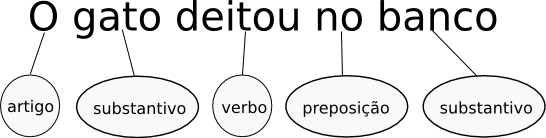
\includegraphics[scale=0.5]{img/exemplo_classificacao}
  \end{center}
\end{figure}

Nosso trabalho consiste em classificar palavras de acordo com seu contexto, ou seja, é feita a análise em termos das unidades primitivas que a compõem, e uma vez que ela é cumprida, podemos passar para outras análises como a sintática ou semântica.


%------------------------------------------------------------------------------
\section{Objetivo}\label{sec:objetivo}
%------------------------------------------------------------------------------

Este trabalho tem, por fim, propor um novo método de classificação de palavras em classes gramáticais e analisar sua eficiência em relação a trabalhos já publicados que utilizam métodos já consolidados. Isso apenas para o escopo da língua portuguesa brasileira. 

Para buscar uma boa eficiência será proposto um método novo que se baseia em classificar primeiramente palavras mais fáceis (\textit{e.g verbos}), desse modo, espera-se deixar palavras ambíguas por último. Por exemplo, para a \autoref{fig:exemploclassificacao} deixaríamos a palavra \textit{banco} por último, uma vez que não sabemos do que isso se trata semanticamente.  

Como já mencionado, o estado-da-arte de atualmente tem cerca de 97\% de precisão, tentaremos ultrapassar esse limite aplicando técnicas novas e utilizando características das palavras variadas, como por exemplo a escolha de diferentes características à serem levadas em consideração no momento da classificação. É importante salientar que a precisão da classificação não será a unica medida levada em consideração, assim como o tempo de processamento gasto para cada córpus.

Para exemplificar brevemente, no final pretende-se que o modelo seja capaz de identificar o uso das palavras de acordo com todas suas análises, como mostrado abaixo.

\begin{center}
\textit{homem + coroa = rei}
\end{center}



%------------------------------------------------------------------------------
\section{Estrutura do trabalho}\label{sec:estruturadotrabalho}
%------------------------------------------------------------------------------

A fim de proporcionar uma boa interpretação, esse trabalho foi dividido nos
seguintes capítulos:

\autoref{problema}: Será descrito o problema deste trabalho.

\autoref{fundamentos}: Descreve os principais fundamentos necessários para entender o método proposto.

\autoref{trabalhosrelacionados}: Apresentação de trabalhos relacionados que procuram resolver o mesmo problema utilizando métodos semelhantes que o proposto.

\autoref{desenvolvimento}: Apresentará o método proposto e os componentes utilizados.

\autoref{comparativo}: Fará uma comparação entre os resultados preliminares alcançados através do método proposto, assim como as discussões do mesmo.

\autoref{conclusao}: Apresentará as considerações finais.

